%% ID: discs_on_a_table
%% TITLE: Discs on a Table
%% TYPE: question
%% QUESTIONTYPE: numeric
%% CONCEPTS:  energy, momentum, vectors
%% VIDEOS: 
%% LEVEL: 6
%% TOPIC: mechanics/dynamics
%% ORDER: 4

\begin{hint}[Discs on a Table]%[A1989FMsQ8a] %Very heavily adapted, pretty much unrecognisable; the Coefficient of Restitution has been completely purged.
{A table top is in the form of a smooth horizontal rectangle ABCD with AB = $a$, BC = $b$ where $a>b$. A small circular disc $P$ of mass $m$ is at rest at the centre of the table. An identical disk $Q$ is projected with speed $u$ along the table top in a direction parallel to AB and collides with $P$. After the collision $P$ and $Q$ move directly towards B and C respectively.
\begin{enumerate}
	\item Draw diagrams illustrating the situation before and after the collision both the frame of the table and in the zero momentum frame (ZMF).
\end{enumerate}
The loss of kinetic energy in the collision is \begin{equation*} \frac{(a^{2} - b^{2}) mu^{2}}{4a^{2}} \end{equation*}
\begin{enumerate}[resume]
	\item Show that the discs reach B and C simultaneously, and find the time from the collision until $Q$ reaches C.
	
\end{enumerate}
}
{The zero momentum frame (ZMF) is a set of axes moving such that the total momentum of the objects being considered is zero. To transform into it, subtract the speed of the centre of mass of the bodies. It is defined in terms of vectors, but here we only need the 1D form:  $v_{\textrm{ZMF}} = \frac{m_{1}v_{1} + m_{2}v_{2}}{m_{1} + m_{2}}$ in the direction of $v_{1}$ and $v_{2}$. The ZMF is sometimes called the Centre of Mass frame, since in it the Centre of Mass is fixed.}
{\textit{Adapted with permission from UCLES, A Level Further Mathematics, June~1989, Syllabus~C, Special~Paper, Question~8.}}
{\begin{enumerate}
	\item It is easiest to draw the diagrams as one big table, showing the system in the ZMF below the system in the table frame as rows and the before/after state as the columns, as in Figure \ref{fig:Dynamics_ZMF_table_collision}. When drawing a diagram like this one, it is standard to draw the initial table frame, then the initial ZMF, then final ZMF and then back into the table frame to get the final answer; but here we know the final and initial state in the table frame and it is the ZMF frame we are interested in.
\begin{figure}[h]
\centering
\includegraphics[width=0.9\textwidth]{Dynamics_ZMF_table_collision}
\caption{}
\label{fig:Dynamics_ZMF_table_collision}
\end{figure}

Before the collision in the table frame, cell $(1)$ in Figure \ref{fig:Dynamics_ZMF_table_collision}, disc $Q$ is moving towards $P$ with speed $u$ and $P$ is stationary at the centre of the table. The collision must be oblique (not head on) in order for the discs to go off at angles to one another and make this a 2D collision. After the collision in the table frame, cell $(4)$, both discs are both moving at an angle $\theta = \arctan(\frac{b}{a})$ to the horizontal.

To transform into the ZMF we need to find the speed of the ZMF, $v_{\textrm{ZMF}} = \frac{m_{1}v_{1} + m_{2}v_{2}}{m_{1} + m_{2}}$ for two discs moving along a line. Here we find $v_{\textrm{ZMF}} = \frac{u}{2}$ and so we subtract this from the velocity of everything. The table is then also moving backwards at $\frac{u}{2}$, as indicated at the bottom of both cells in Figure \ref{fig:Dynamics_ZMF_table_collision}, but this does not affect the system. Once $v_{\textrm{ZMF}}$ has been subtracted, we get the situation in Figure \ref{fig:Dynamics_ZMF_table_collision} cell $(2)$.
After the collision in the ZMF both discs must have the same speed, $v$, in opposite directions and at some angle $\phi$ with with direction DA, in order that momentum be zero and energy be conserved. Since the masses are equal, moving in opposite directions at the same speed will sum to zero momentum and the kinetic energy loss is (probably) not total so they must have a non-zero speed. It will become clear later that $\phi$ is in fact $0$, but for now an arbitrary angle will suffice; since any direction will give a total momentum of zero.

	\item The simplest way to show the two discs arrive at the corners simultaneously is to consider their speeds: if they are equal, then the time taken for them to travel the diagonal (the same length for both discs) will be equal and so they arrive at the same time, $t$, which needs to be found.

It is clear that initially there is no momentum parallel to DA, and so conservation of momentum in that direction gives:
\begin{align*} 0 &= mv_{Q} \sin(\theta) - mv_{P}\sin(\theta) \\ mv_{Q}\sin(\theta) &= mv_{P}\sin(\theta) \\ v_{P} &= v_{Q} \\ &= v_{f}\end{align*}
so the final speeds are equal and they arrive at the corners simultaneously. We shall call their speed $v_{f}$, but we still need to find it in terms of $u$.

We can achieve this by finding $v$, as labelled in Figure \ref{fig:Dynamics_ZMF_table_collision}, the speed of both discs after the collision in the ZMF. To do this, consider the kinetic energy before and after the collision (in the ZMF; kinetic energy is not the same in all frames, only changes in KE are unchanged across frames):
\begin{align*} \left[ \textrm{Initial KE} \right] - \left[ \textrm{KE Loss}\right] &= \left[ \textrm{Final KE} \right] \\
\left[ \frac{1}{2}(m)\left(\frac{u}{2}\right)^{2} + \frac{1}{2}(m)\left(\frac{u}{2}\right)^{2} \right] - \left[\frac{(a^{2} - b^{2})mu^{2}}{4a^{2}}\right] &= \left[ \frac{1}{2}mv^{2} + \frac{1}{2}mv^{2}\right]\end{align*}
divide through by $\frac{1}{2}mu^{2}$:
\begin{align*} \left( \frac{1}{4} + \frac{1}{4} \right) - \left( \frac{a^{2} - b^{2}}{2a^{2}} \right) &= \left( \frac{v^{2}}{u^{2}} + \frac{v^{2}}{u^{2}} \right) \\
\frac{b^2}{2a^{2}} &= \frac{2v^{2}}{u^{2}} \end{align*}
and so the final speed of both particles in the ZMF is
\begin{equation*} v = \sqrt{\frac{b^{2}u^{2}}{4a^{2}}} = \frac{b}{2a} u \end{equation*}

Consider the velocities now, since these add as vectors and take into account the directions involved. We know the direction in the table frame and we know the velocity of the ZMF. Adding the velocity of the ZMF back onto the velocities of the discs, as in Figure \ref{fig:Dynamics_ZMF_velocity_add}, gives the direction of the velocities in the table frame. We know that the angle from the resultant velocity to the $x$-direction (in the diagram) must be $\theta$ for both discs, because velocity points along the direction of motion. Since $v_{P} = v_{Q}$, we have 3 sides the same and so the triangles must be similar. Looking at the angle from the ZMF velocity to $v$ for the two discs, it must be the same and so similar triangles requires $90^{\circ} + \phi = 90^{\circ} - \phi$, which can only be true if $\phi$ is zero.

\begin{figure}[h]
\centering
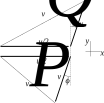
\includegraphics[width=0.3\textwidth]{Dynamics_ZMF_velocity_add}
\caption{}
\label{fig:Dynamics_ZMF_velocity_add}
\end{figure}

Thus the triangles are right-angled, and so $v_{P} = v_{Q} = v_{f}$ can be found by Pythagoras' Theorem:
\begin{align*} v_{f} &= \sqrt{ v^{2} + \left(\frac{u}{2}\right)^{2}} \\ &= \sqrt{ \frac{b^{2}u^{2}}{4a^{2}} + \frac{u^{2}}{4}} \\ &= \frac{\sqrt{a^{2} + b^{2}}}{2a} u \end{align*}
This could all be done without the ZMF, since in this case the direction in the table frame was given initially; but it is good practise in using the ZMF.

The time taken is $t = \frac{d}{v_{f}}$ where $d$ is the length from the centre of the table to the corner. Again Pythagoras' Theorem can be used:
\begin{align*} d &= \sqrt{ \left(\frac{a}{2}\right)^{2} + \left(\frac{b}{2}\right)^{2} } \\ &= \sqrt{\frac{1}{4}(a^{2} + b^{2})} \\ &= \frac{1}{2}\sqrt{a^{2} + b^{2}} \end{align*}
and so we can find $t$, the time taken for $Q$ to reach C:
\begin{align*} t = \frac{d}{v_{f}} = \frac{\frac{1}{2}\sqrt{a^{2} + b^{2}}}{\left(\frac{\sqrt{a^{2} + b^{2}}}{2a} u\right)} = \frac{a}{u} \end{align*}

\end{enumerate}
}
\end{hint}